\subsection{Tutorial 1: Lennard-Jones fluid}
\label{lennard-jones-label}

\begin{figure}
{\centering
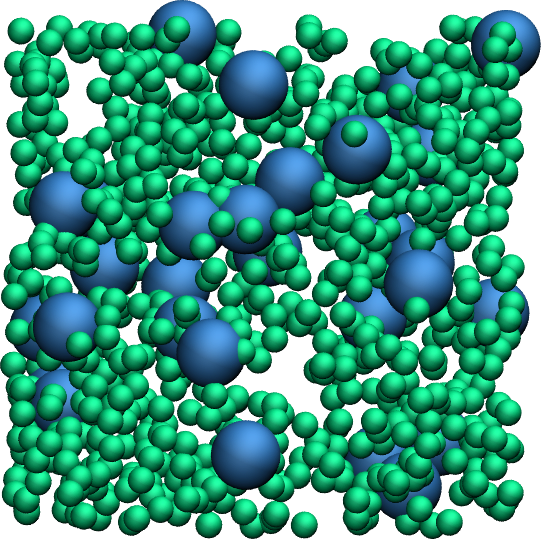
\includegraphics[width=0.55\linewidth]{binary_LJ_fluid}
\caption{Snapshot of the Lennard-Jones fluid made using VMD, with both types of atoms represented as spheres.}}
\label{fig:binary_LJ_fluid}
\end{figure}

\noindent The objective of this tutorial is to perform the simulation of a binary fluid using LAMMPS. The system is a Lennard-Jones fluid made of neutral particles with two different diameters in a cubic box with periodic boundary conditions (Fig.~\ref{fig:binary_LJ_fluid}). The temperature of the system is maintained using a Langevin thermostat \cite{schneider1978molecular}, and basic quantities are extracted from the system, including the potential and kinetic energies. 

\subsubsection{My first input}

\noindent To run a simulation using LAMMPS, one needs to write a series of commands in an input script. For clarity, this script will be divided into five categories which we are going to fill up one by one. Create a folder, call it \textit{my-first-input/}, and then create a blank text file in it called \textit{input.lammps}. Copy the following lines in \textit{input.lammps}, where a line starting with a brace ($\#$) is a comment that is ignored by LAMMPS:
{\small  \begin{verbatim}
# PART A - ENERGY MINIMIZATION
# 1) Initialization
# 2) System definition
# 3) Simulation settings
# 4) Visualization
# 5) Run
\end{verbatim}}
\noindent These five categories are not required in every input script, and should not necessarily be in that exact order. For instance, parts 3 and 4 could be inverted, or part 4 could be omitted. Note however that LAMMPS reads input files from top to bottom, therefore the \textit{Initialization} and \textit{System definition} categories must appear at the top of the input, and the \textit{Run} category at the bottom.

\paragraph{System initialization}
In the first section of the script, called \textit{Initialization}, let us indicate to LAMMPS the most basic information about the simulation, such as:
\begin{itemize}
\item the conditions at the boundaries of the box (e.g. periodic or non-periodic),
\item the type of atoms (e.g. uncharged single dots or spheres with angular velocities).
\end{itemize}
Enter the following lines in \textit{input.lammps}:
{\small \begin{verbatim}
# 1) Initialization
units lj
dimension 3
atom_style atomic
pair_style lj/cut 2.5
boundary p p p
\end{verbatim}}
The first line, \textit{units lj}, indicates that we want to use the system of unit called \textit{LJ}, for Lennard-Jones, for which all quantities are unitless. The second line, \textit{dimension 3}, indicates that the simulation is 3D. The third line, \textit{atom$\_$style atomic}, that the \textit{atomic} style
will be used, therefore each atom is just a dot with a mass. The fourth line, \textit{pair$\_$style lj/cut 2.5}, indicates that atoms will be interacting through a Lennard-Jones potential with a cut-off equal to $r_c = 2.5$ (unitless) \cite{wang2020lennard,fischer2023history}:
$$E_{ij} (r) = 4 \epsilon_{ij} \left[ \left( \dfrac{\sigma_{ij}}{r} \right)^{12} - \left( \dfrac{\sigma_{ij}}{r} \right)^{6} \right], ~ \text{for} ~ r < r_c,$$
where $r$ is the inter-particles distance, $\epsilon_{ij}$ the depth of potential well that sets the interaction strength, and $\sigma_{ij}$ the distance parameter, or particle effective size. Here, the indexes \textit{ij} refer to the particle types \textit{i} and \textit{j}. The last line, \textit{boundary p p p}, indicates that the periodic boundary conditions will be used along all three directions of space (the 3 \textit{p} stand for \textit{x}, \textit{y}, and \textit{z}, respectively).

\paragraph{System definition}
Let us fill the \textit{System definition} category of the input script:
{\small \begin{verbatim}
# 2) System definition
region simulation_box block -20 20 -20 20 -20 20
create_box 2 simulation_box
create_atoms 1 random 1500 341341 simulation_box
create_atoms 2 random 100 127569 simulation_box
\end{verbatim}}
\noindent The first line, \textit{region simulation$\_$box (...)}, creates a region named \textit{simulation$\_$box} that is a block (i.e. a rectangular cuboid) that extends from -20 to 20 (no unit) along all 3 directions of space. The second line, \textit{create$\_$box 2 simulation$\_$box}, creates a simulation box based on the region \textit{simulation$\_$box} with \textit{2} types of atoms. The third line, \textit{create$\_$atoms (...)} creates 1500 atoms of type 1 randomly within the region \textit{simulation$\_$box}. The integer \textit{341341} is a seed that can be changed in order to create different
initial conditions for the simulation. The fourth line creates 100 atoms of type 2.

\paragraph{Simulation Settings}
Let us fill the \textit{Simulation Settings} category section of the \textit{input} script:
{\small \begin{verbatim}
# 3) Simulation settings
mass 1 1
mass 2 1
pair_coeff 1 1 1.0 1.0
pair_coeff 2 2 0.5 3.0
\end{verbatim}}
The two first commands, \textit{mass (...)}, attribute a mass equal to 1 (unitless) to both atoms of type 1 and 2. Alternatively, one could have written these two commands into one single line: \textit{mass $\star 1$}, where the star symbol means \textit{all} the atom types of the simulation.  The third line, \textit{pair$\_$coeff 1 1 1.0 1.0}, sets the Lennard-Jones coefficients for the interactions between atoms of type 1, respectively the energy parameter $\epsilon_{11} = 1.0$ and the distance parameter $\sigma_{11} = 1.0$. Similarly, the last line sets the Lennard-Jones coefficients for the interactions between atoms of type 2, $\epsilon_{22} = 0.5$, and $\sigma_{22} = 3.0$. By default, LAMMPS calculates the cross coefficients between the different atom types using geometric average: $\epsilon_{ij} = \sqrt{\epsilon_{ii} \epsilon_{jj}}$, $\sigma_{ij} = \sqrt{\sigma_{ii} \sigma_{jj}}$. 

\paragraph{Energy minimization}
The system is now fully parametrized. Let us fill the two last remaining sections by adding the following lines to \textit{input.lammps}:
\begin{verbatim}
# 4) Visualization
thermo 10
thermo_style custom step temp pe ke etotal press

# 5) Run
minimize 1.0e-4 1.0e-6 1000 10000
\end{verbatim}
The \textit{thermo} command asks LAMMPS to print thermodynamic information (e.g. temperature, energy) in the terminal every given number of steps, here 10 steps. The \textit{thermo$\_$style custom} requires LAMMPS to print the system temperature (\textit{temp}), potential energy (\textit{pe}), kinetic energy (\textit{ke}), total energy (\textit{etotal}), and pressure (\textit{press}). Finally, the \textit{minimize} line asks LAMMPS to perform an energy minimization of the system. By default, LAMMPS uses the conjugate gradient (CG) algorithm \cite{hestenes1952methods}.

Run the simulation by typing in a terminal:
\begin{verbatim}
lmp -in input.lammps
\end{verbatim}
where the command \textit{lmp} is linked to a compiled version of LAMMPS. As the simulation progresses, the potential energy can be seen to decrease from a large positive value to to a negative value. The initially large and positive value of the potential energy was expected because the atoms have been created at random positions within the simulation box and some of them are probably overlapping, resulting in a large initial energy which is the consequence of the repulsive part of the Lennard-Jones interaction potential. As the energy minimization progresses, the energy rapidly decreases and reaches a negative value, indicating that the atoms have been displaced at reasonable distances from each other.

\paragraph{Molecular dynamics}
The system is now ready. Let us continue filling up the input script and adding commands to perform a molecular dynamics simulation that will start from the final state of the previous energy minimization step. In the same input script, after the \textit{minimization} command, add the following
lines:
\begin{verbatim}
# PART B - MOLECULAR DYNAMICS
# 4) Visualization
thermo 50
\end{verbatim}
Since LAMMPS reads the input from top to bottom, these lines will be executed after the energy minimization. There is no need to re-initialize or re-define the system. The \textit{thermo} command is called a second time within the same input, so the previously entered value of 10 will be replaced by
the value of 50 as soon as \textit{PART B} starts. Then, let us add a second \textit{Run} section:
\begin{verbatim}
# 5) Run
fix mynve all nve
fix mylgv all langevin 1.0 1.0 0.1 1530917
timestep 0.005
run 10000
\end{verbatim}
The \textit{fix nve} is used to update the positions and the velocities of the atoms in the group \textit{all} at every step. The group \textit{all} is a default group that contains every atom. The second fix applies a Langevin thermostat to the atoms of the group \textit{all}, with a desired initial temperature of 1.0 (unitless), and a final temperature of 1.0 as well \cite{schneider1978molecular}. A \textit{damping} parameter of 0.1 is used. The \textit{damping} parameter determines how rapidly the temperature is relaxed to its desired value. The number \textit{1530917} is a seed, you can change it to perform statistically independent simulations. Finally, the last two lines set the value of the \textit{timestep} and the number of steps for the *run*, respectively, corresponding to a total duration of 50 (unitless).

Run the simulation again using LAMMPS. {\color{red}From the log file}, one can see that the temperature \textit{Temp} starts from 0, but rapidly reaches the requested value and stabilize itself near $T=1$ (unitless). \vspace{0.25cm} \noindent From what has been printed in the \textit{log} file, one can plot the potential energy ($p_\text{e}$) and the kinetic energy ($k_\text{e}$) of the system over time {\color{red}(see the figure below)}.

{\color{red}Figure: a) The potential energy ($p_\text{e}$) rapidly decreases during energy minimization (orange). Then, after the molecular dynamics simulation starts, $p_\text{e}$ increases until it reaches a plateau value of about -0.25 (blue). b) The kinetic energy ($k_\text{e}$) is equal to zero during energy minimization, then increases during molecular dynamics until it reaches a plateau value of about 1.5.}

\paragraph{Trajectory visualization}

 To visualize the trajectories of the atoms, we first need to print the positions of the atoms in a file at a regular interval. Add the following command to the \textit{input.lammps} file, in the \textit{Visualization} section of \textit{PART B}:
\begin{verbatim}
dump mydmp all atom 100 dump.lammpstrj
\end{verbatim}
Run the \textit{input.lammps} using LAMMPS again. The file named \textit{dump.lammpstrj} created by LAMMPS within \textit{my-first-input/} can be opened using VMD.

\subsubsection{Improving the script}

Let us improve the input script and perform slightly more advanced operations, such as imposing a specific initial
positions to the atoms, and restarting the simulation from a previously saved configuration. 

\paragraph{Control the initial atom positions}
\noindent Create a new folder next to \textit{my-first-input/}, and call it \textit{improved-input/}. Then, create a new input file within \textit{improved-input/} and call it \textit{input.min.lammps}. Similarly to what has been done previously, copy the following lines into \textit{input.min.lammps}:
\begin{verbatim}
# 1) Initialization
units lj
dimension 3
atom_style atomic
pair_style lj/cut 2.5
boundary p p p
\end{verbatim}
To create the atoms of types 1 and 2 in two separate regions, let us create three separate regions: A cubic region for the simulation box and two additional regions for placing the atoms:
\begin{verbatim}
# 2) System definition
region simulation_box block -20 20 -20 20 -20 20
create_box 2 simulation_box
region cylinder_in cylinder z 0 0 10 INF INF side in
region cylinder_out cylinder z 0 0 10 INF INF side out
create_atoms 1 random 1000 341341 cylinder_out
create_atoms 2 random 150 127569 cylinder_in
\end{verbatim}
The \textit{side in} and \textit{side out} keywords are used to define regions that are respectively inside and outside of the cylinder of radius 10. Then, copy similar lines as previously into \textit{input.min.lammps}:
\begin{verbatim}
# 3) Simulation settings
mass 1 1
mass 2 1
pair_coeff 1 1 1.0 1.0
pair_coeff 2 2 0.5 3.0

# 4) Visualization
thermo 10
thermo_style custom step temp pe ke etotal press
dump mydmp all atom 10 dump.min.lammpstrj

# 5) Run
minimize 1.0e-4 1.0e-6 1000 10000
write_data minimized_coordinate.data
\end{verbatim}
The main novelty, compared to the previous input script, is the \textit{write$\_$data} command. This command is used to print the final state of the simulation in a file named \textit{minimized$\_$coordinate.data}. Note that the \textit{write$\_$data} command is placed after the \textit{minimize} command. This \textit{.data} file will be used later to restart the simulation from the final state of the energy minimization step.

Run the \textit{input.min.lammps} script using LAMMPS. A new dump file named \textit{dump.min.lammpstrj} will appear in the folder, allowing you to visualize
the atom's trajectories during minimization. In addition, a file named \textit{minimized$\_$coordinate.data} will be created. If you open \textit{minimized$\_$coordinate.data} with a text editor, you can see that it contains all the information necessary to restart the simulation, such as the number of atoms and the box size, the \textit{masses}, the \textit{pair$\_$coeffs}.
The \textit{minimized$\_$coordinate.data} file also contains the final positions of the atoms within the \textit{Atoms} section.
The first five columns of the \textit{Atoms} section correspond (from left to right) to the atom indexes (from 1 to the total number of atoms, 1150), the atom types (1 or 2 here), and the atoms positions $x$, $y$, $z$. The last three columns are image flags that keep track of which atoms crossed the periodic boundary.

\paragraph{Restarting from a saved configuration}
Let us create a new input file and start a molecular dynamics simulation directly from the previously saved configuration. Within \textit{improved-input/}, create a new file named \textit{input.md.lammps} and copy the same lines as previously:
\begin{verbatim}
# 1) Initialization
units lj
dimension 3
atom_style atomic
pair_style lj/cut 2.5
boundary p p p
\end{verbatim}
Here, instead of creating a new region and adding atoms to it, we can simply import the previously saved configuration by adding the following command to \textit{input.md.lammps}:
\begin{verbatim}
# 2) System definition
read_data minimized_coordinate.data
\end{verbatim}
By visualizing the previously generated \textit{dump.min.lammpstrj} file, you may have noticed that some atoms have moved from one region to the other during minimization. To start the simulation from a clean slate, with only atoms of type 2 within the cylinder and atoms of type
1 outside the cylinder, let us delete the misplaced atoms by adding the following commands to \textit{input.md.lammps}:
\begin{verbatim}
read_data minimized_coordinate.data
region cylinder_in cylinder z 0 0 10 INF INF side in
region cylinder_out cylinder z 0 0 10 INF INF side out
group group_type_1 type 1
group group_type_2 type 2
group group_region_in region cylinder_in
group group_region_out region cylinder_out
group group_type_1_in intersect group_type_1 group_region_in
group group_type_2_out intersect group_type_2 group_region_out
delete_atoms group group_type_1_in
delete_atoms group group_type_2_out
\end{verbatim}
The two first \textit{region} commands recreate the previously defined regions, which is necessary since regions are not saved by the \textit{write$\_$data} command. The first two \textit{group} commands create atom groups based on their types. The next two \textit{group} commands create atom groups based on their
positions at the beginning of the simulation, i.e. when the commands are being read by LAMMPS. The last two \textit{group} commands create atom groups based on the intersection between the previously defined groups. Finally, the two \textit{delete$\_$atoms} commands delete the atoms of type 1 that are located within the cylinder, as well as the atoms of type 2 that are located outside the cylinder, respectively. 

{\color{red}When you run the \textit{input.md.lammps} input using LAMMPS, you can see in the \textit{log} file how many atoms are in each group, and how many atoms have been deleted:}
\begin{verbatim}
1000 atoms in group group_type_1
150 atoms in group group_type_2
149 atoms in group group_region_in
1001 atoms in group group_region_out
0 atoms in group group_type_1_in
1 atoms in group group_type_2_out
Deleted 0 atoms, new total = 1150
Deleted 1 atoms, new total = 1149
\end{verbatim}
Add the following lines to \textit{input.md.lammps}. Note the absence of \textit{Simulation settings} section, because the settings are taken from the \textit{.data} file.
\begin{verbatim}
# 4) Visualization
thermo 1000
dump mydmp all atom 1000 dump.md.lammpstrj
\end{verbatim}
Let us extract the number of atoms of each type inside the cylinder as a function of time, by adding the following commands to \textit{input.md.lammps}:
\begin{verbatim}
variable number_type1_in &
    equal count(group_type_1,cylinder_in)
variable number_type2_in & 
    equal count(group_type_2,cylinder_in)
fix myat1 all ave/time 10 200 2000 &
    v_number_type1_in &
    file output-population1vstime.dat
fix myat2 all ave/time 10 200 2000 &
    v_number_type2_in &
    file output-population2vstime.dat
\end{verbatim}
The 2 \textit{variables} are used to count the number of atoms of a specific group in the \textit{cylinder$\_$in} region. The two \textit{fix ave/time} are calling the previously defined variables and are printing their values into text files. By using \textit{10 200 2000}, variables are evaluated every 10 steps, averaged 200 times, and printed in the \textit{.dat} files every 2000 steps.

\begin{figure}
\centering
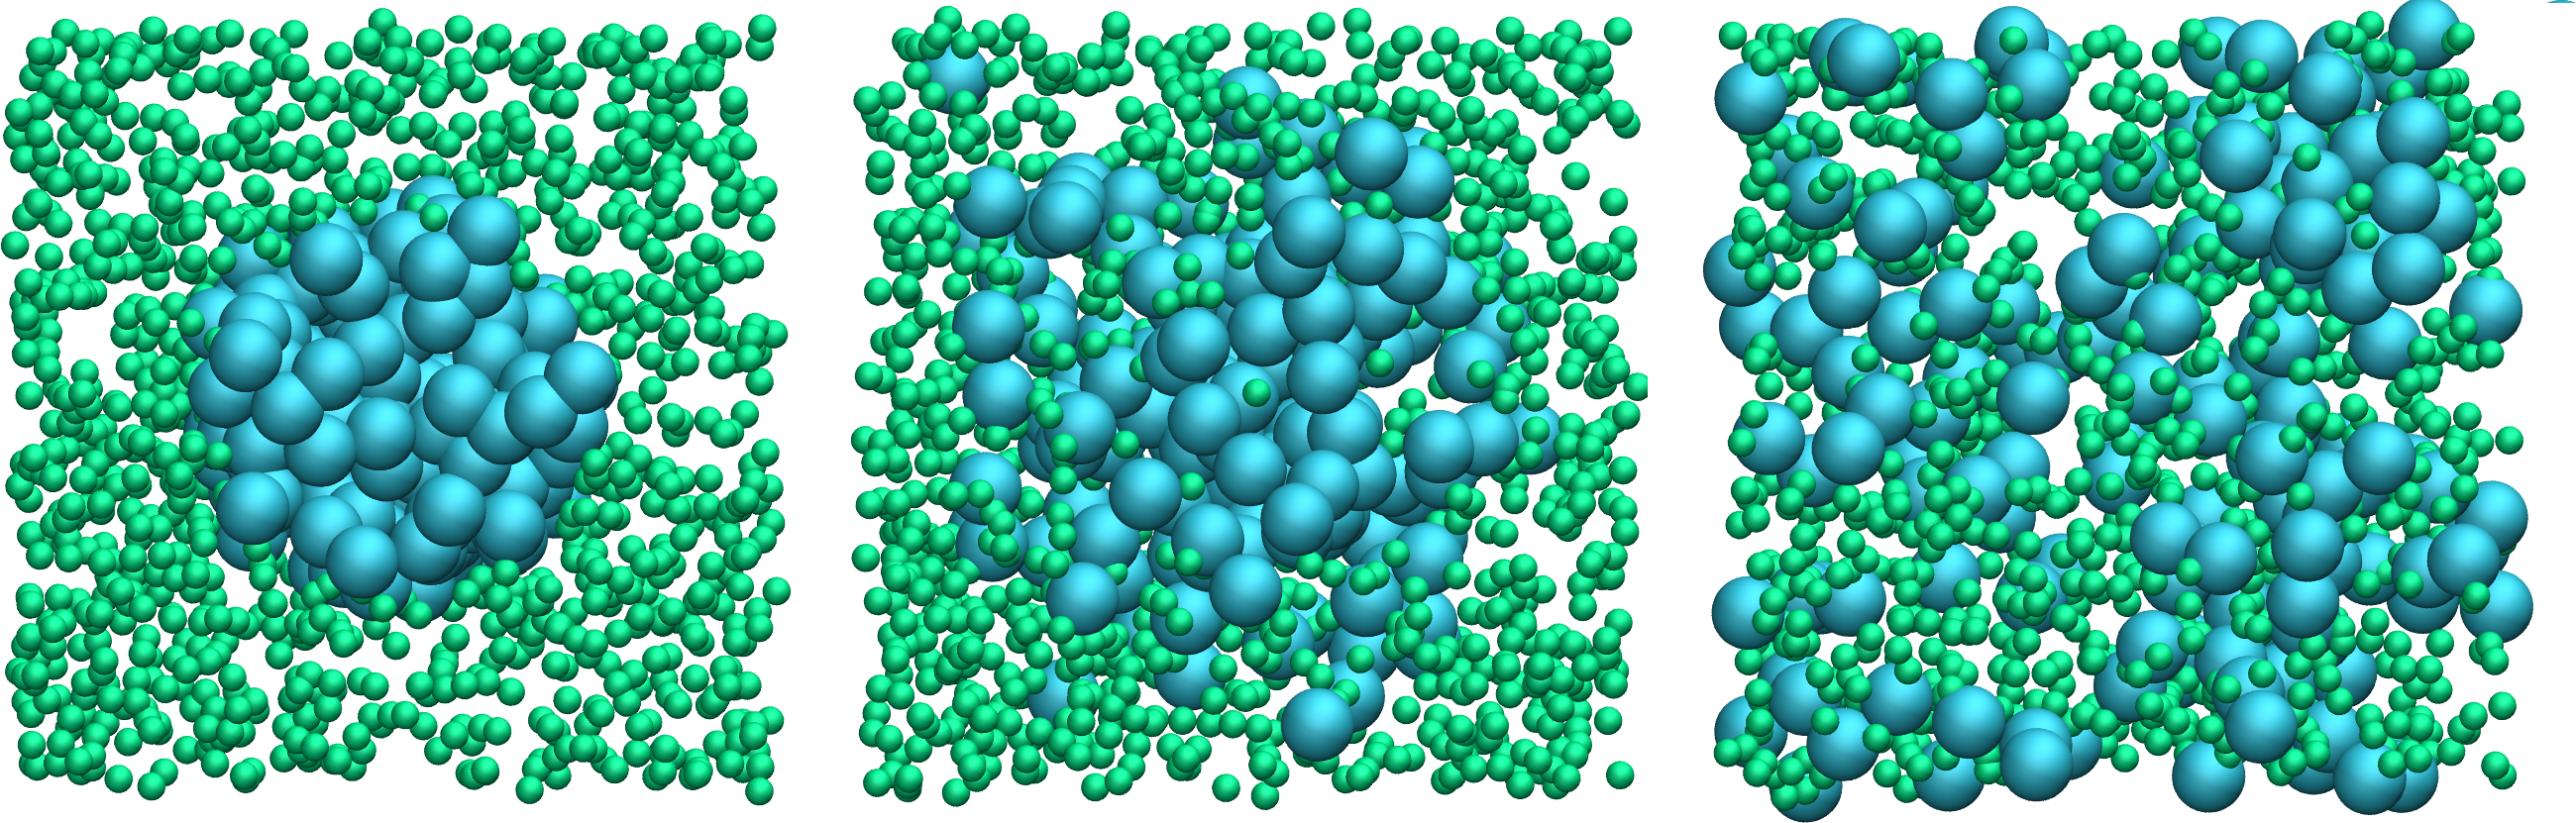
\includegraphics[width=\linewidth]{evolution}
\caption{Evolution of the system during mixing.}
\label{fig:evolution-population}
\end{figure}

Let us also extract the coordination number per atom between atoms of type 1 and 2, i.e. the average number of atoms of type 2 in the vicinity of the atoms of type 1. This coordination number will be used as an indicator of the degree of mixing of our binary mixture. Add the following lines into \textit{input.md.lammps}:
\begin{verbatim}
compute coor12 group_type_1 coord/atom &
    cutoff 2.0 group group_type_2
compute sumcoor12 all reduce ave c_coor12
fix myat3 all ave/time 10 200 2000 &
    c_sumcoor12 file coordinationnumber12.dat
\end{verbatim}
The \textit{compute ave} is used to average the per atom coordination number that is calculated by the \textit{coord/atom} compute. This averaging is necessary as \textit{coord/atom} returns an array where each value corresponds to a certain couple of atoms i-j. Such an array can't be printed by \textit{fix ave/time}. Finally, let us complete the script by adding the following lines to \textit{input.md.lammps}:
\begin{verbatim}
# 5) Run
velocity all create 1.0 4928459 mom yes rot yes &
    dist gaussian
fix mynve all nve
fix mylgv all langevin 1.0 1.0 0.1 1530917 zero yes
timestep 0.005
run 300000
write_data mixed.data
\end{verbatim}
There are a few differences from the previous simulation. First, the \textit{velocity create} command attributes an initial velocity to every atom.
The initial velocity is chosen so that the average initial temperature is equal to 1 (unitless). The additional keywords ensure that no linear momentum (\textit{mom yes}) and no angular momentum (\textit{rot yes}) are given to the system and that the generated velocities are distributed as a Gaussian. Another improvement is the \textit{zero yes} keyword in the Langevin thermostat, which ensures that the total random force is equal to zero.
Run \textit{input.md.lammps} using LAMMPS. Open the \textit{dump.md.lammpstrj} using VMD to observe the mixing of the two populations as the time evolves (Fig.\,\ref{fig:evolution-population}). The generated \textit{.dat} files indicate the number of atoms in each region as a function time (Fig.\,\ref{fig:mixing}\,a). In addition, as the mixing progresses, the calculated coordination number increases from about $0.01$ to $0.35$ (Fig.\,\ref{fig:mixing}\,b).

\begin{figure}
\centering
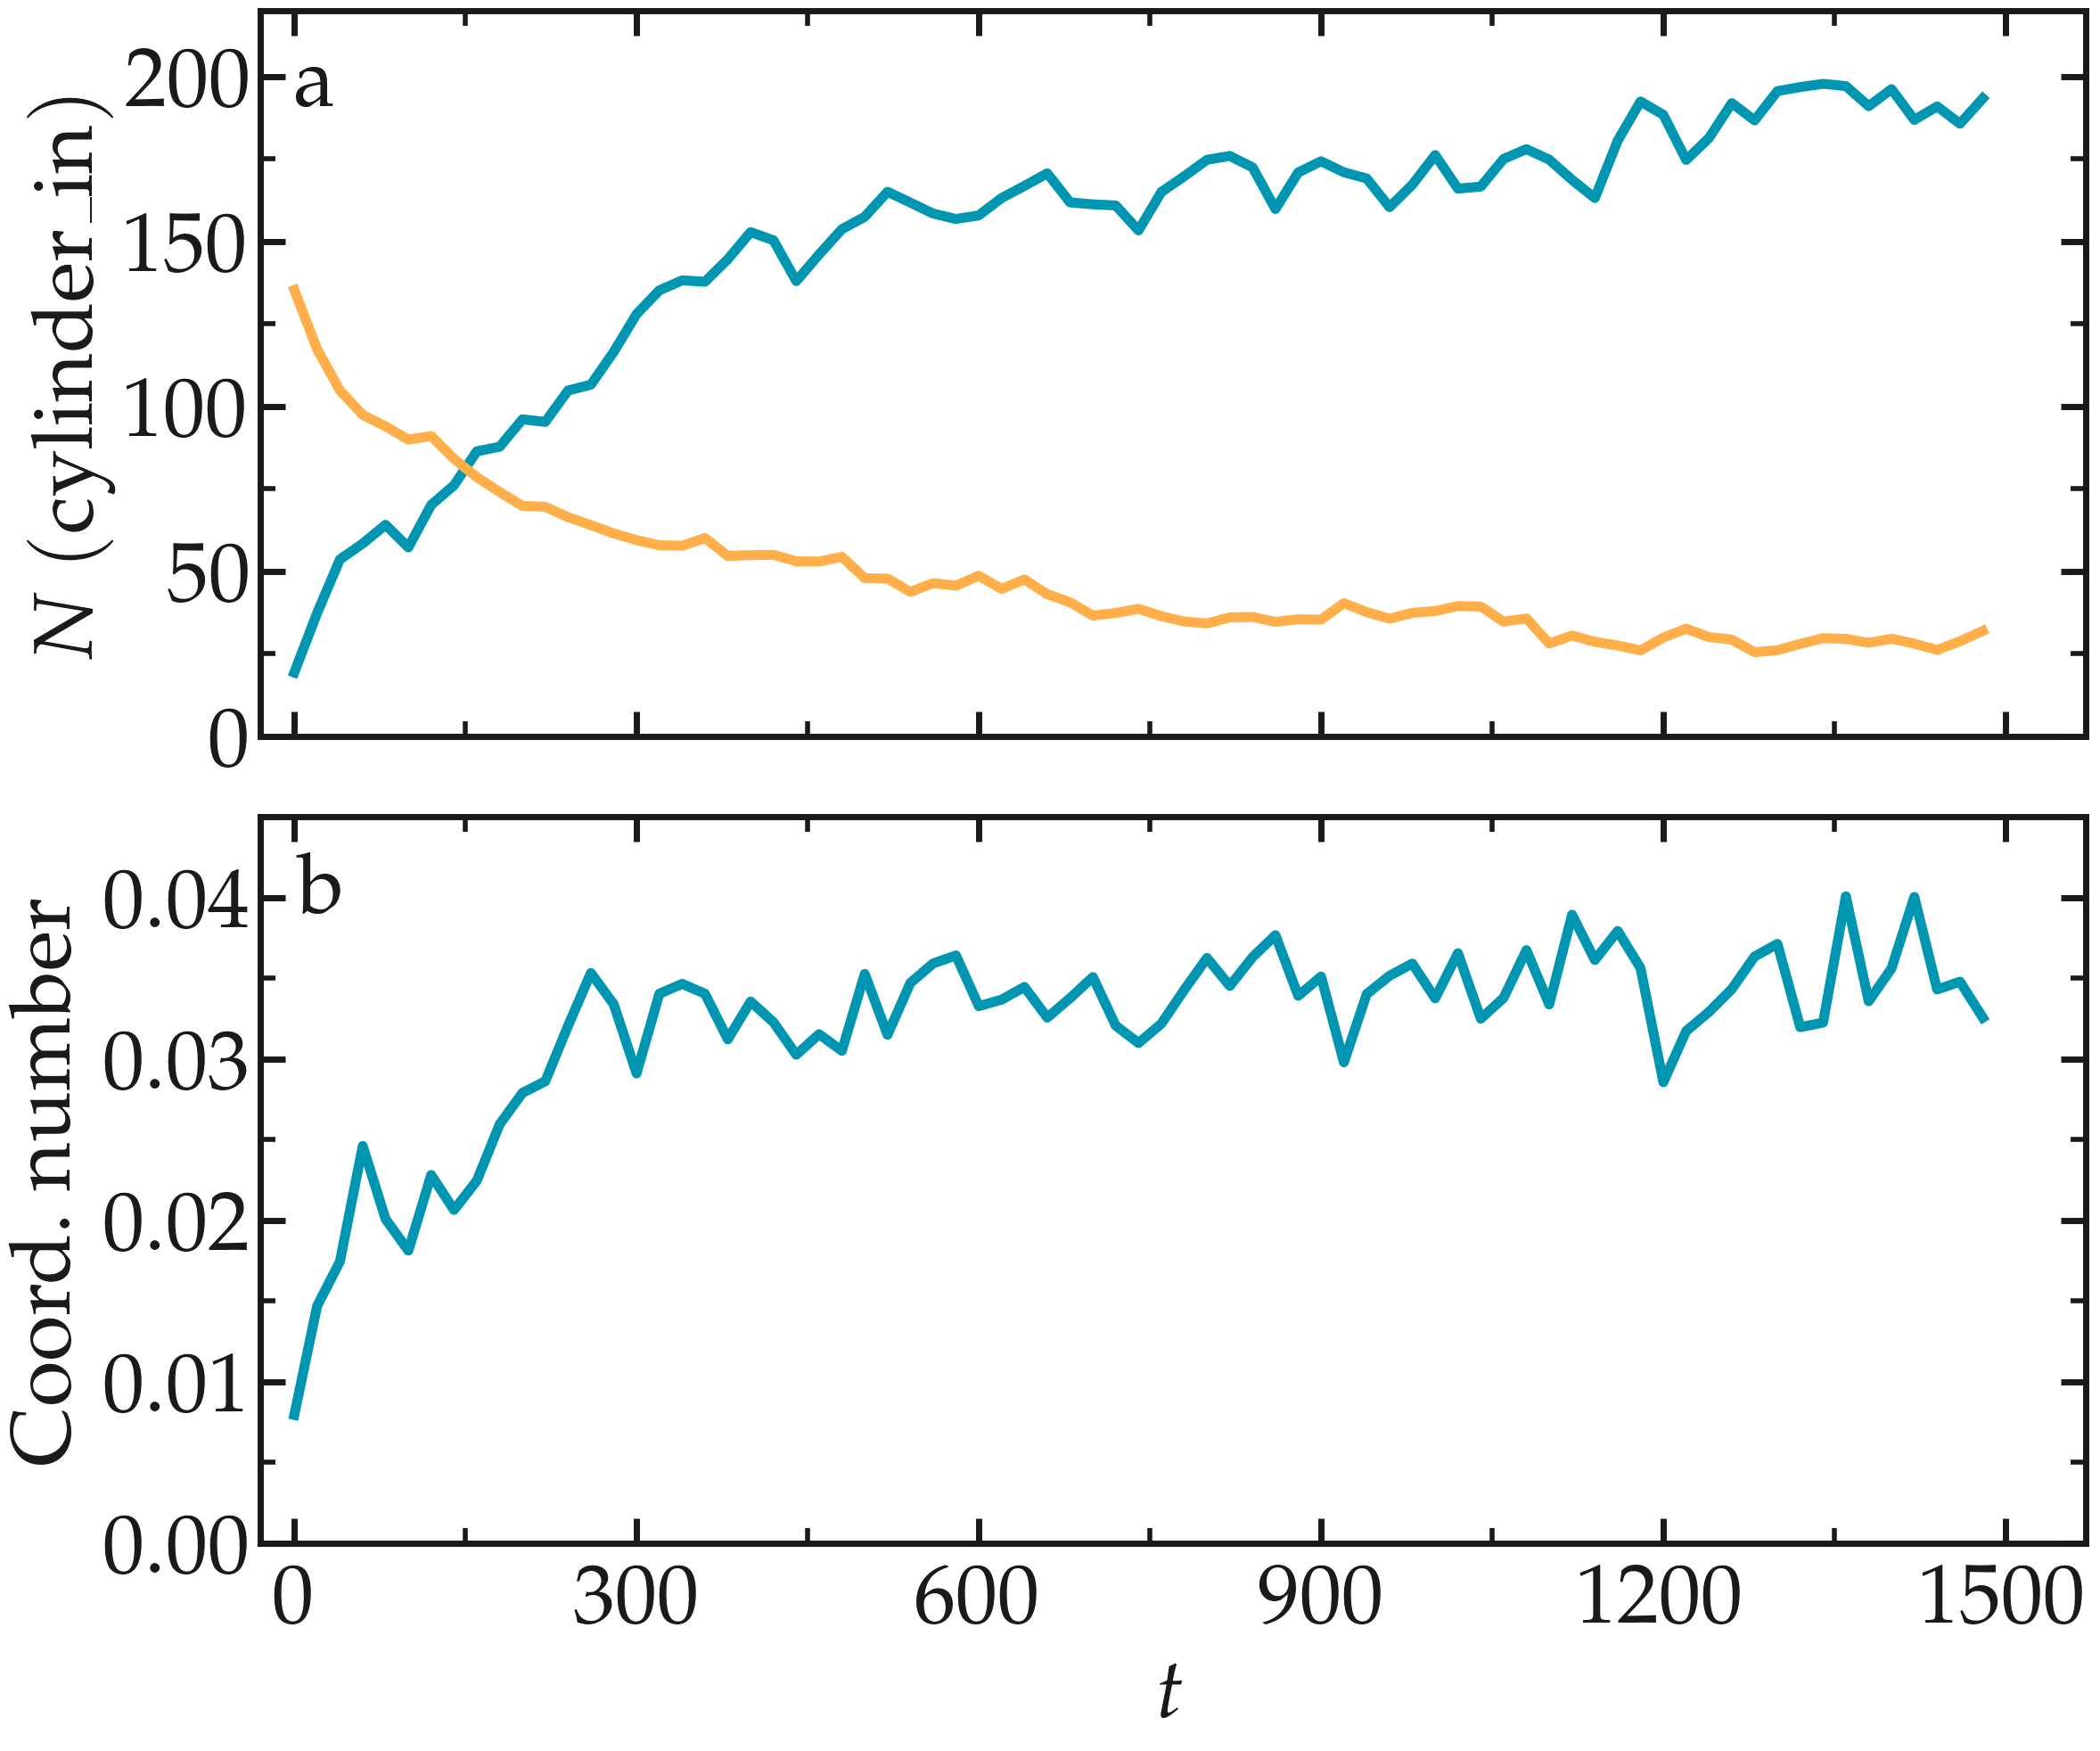
\includegraphics[width=\linewidth]{mixing}
\caption{a) Evolution of the number $N$ of atoms within the \textit{cylinder$\_$in} region as a function of the time $t$. b) Evolution of the coordination number.}
\label{fig:mixing}
\end{figure}

